\documentclass[main.tex]{subfiles}

\begin{document}

\lstset{
  basicstyle=\ttfamily\small,
  backgroundcolor=\color{gray!10},
  frame=single,
  breaklines=true,
  breakindent=0pt,
  xleftmargin=2em,
  framexleftmargin=1em,
  literate=
    {é}{{\'e}}1 {è}{{\`e}}1 { ê}{{\^e}}1 {à}{{\`a}}1 {ç}{{\c{c}}}1
    {’}{{'}}1 {‘}{{'}}1
    {“}{{\textquotedbl}}1 {”}{{\textquotedbl}}1
    {"}{{\textquotedbl}}1
    {_}{{\_}}1
    {→}{{$\rightarrow$}}1
}

\section{Partie William Pinalie}

\subsection{Introduction}

Dans le cadre de mon projet informatique, ma mission consiste à concevoir un
système de contrôle automatisé pour un casier à l’aide de servomoteurs. L’objectif
principal est de permettre l’ouverture et la fermeture contrôlées du casier tout en
intégrant une fonctionnalité de sécurité. Le système doit en effet être capable de
détecter toute obstruction, comme la présence d’une main et s’arrêter
automatiquement afin de prévenir tout risque de blessure ou d’endommagement du
mécanisme. Ce projet combine des compétences en programmation, en électronique
embarquée et en gestion de capteurs. J’ai également pris l’initiative d’ajouter des
exécutables permettant de remplacer un servomoteur si nécessaire, afin de renforcer
la flexibilité et la robustesse du système.

\subsection{Guide installation et création du projet}

\subsubsection{Configuration Raspberry :}

\quad Pour réaliser le projet casiers RFID il faut créer un projet Raspberry en c++ sur visual studio. On utilise un projet Debug en ARM64 puis il faut se connecter à la raspberry en ssh parce qu’on utilise l’éditeur de code visual studio code sur Windows et parce que la communication des servomoteurs et des LED que l’on utilisera tout au long du projet se fait par voie série. Pour cela il faut aller dans :

\begin{lstlisting}
outil → option → Multiplateforme → Gestionnaire de connexions →Ajouter →   Nom d’hote : 10.187.52.121
            	Port : 22
            	Nom d’utilisateur : rfid
            	Type d’authentification : mot de passe
            	Mot de passe : rfid
\end{lstlisting}

Le projet est envoyer sur raspberry lorsque l’on génère la solution

\begin{lstlisting}
→ sudo ./lien de l’éxécutable pour éxécuter le fichier.
\end{lstlisting}

Pour pouvoir utiliser le bus série il faut vérifier qu’aucun programme tourne en arrière-plan.

Pour cela il faut installer lsof :

\begin{lstlisting}
sudo apt-get install lsof
sudo lsof /dev/ttyS0  pour vérifié si le bus série est déjà utilisé.
\end{lstlisting}
Si agetty utilise le port série faire la commande :

\begin{lstlisting}
sudo systemctl stop serial-getty@ttyS0.service
// ou sudo systemctl disable serial-getty@ttyS0.service
\end{lstlisting}

\subsection{Présentation des LED}

Pour utiliser la classe LED donnée, il faut inclure pigpio. 

Il faut rajouter dans les paramètres du projet (clic droit sur le nom du projet dans l’explorateur de solution puis propriétés), cliquez sur l’item Editeur de liens puis Entrées. Rajouter dans le champ Dépendances de bibliothèque le mot pigpio puis valider ces changements en cliquant sur le bouton OK. LE PROJET DOIT ÊTRE SOUS LINUX ET RASPBERRY.

Il faut aussi instaler pigpio sur la raspberry.

\begin{lstlisting}
Sudo apt install pigpio
\end{lstlisting}

Si l’initialisation des LEDs ne fonctionne pas c’est peut-être parce que le
programme pigpiod tourne sur la raspberry donc il faut le supprimer.

\begin{lstlisting}
htop : pour voir si pigpiod et en cours d’utilisation
sudo killall pigpiod : pour arrêter le programme
\end{lstlisting}

Les led utilisées pour ce projet sont des grove led rgb chainable v2.0. Ces led fonctionnes via un protocole série synchrone. La led lit les données qui lui sont destinées, puis les transmet à la suivante. Chaque module possède deux ports, IN et OUT permettant un chainage direct. Ces led ont été choisi car elles sont chainables et elles avoir chacune une couleur personnalisée.

\begin{figure}[H]
	\centering
	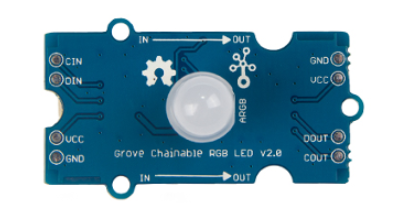
\includegraphics[width=0.8\textwidth]{../images/LED}
	\caption{Led rgb chainable v2.0}
	\label{fig:LED}
\end{figure}

\subsubsection{Branchement des LED}

J’ai branché la led sur le raspberry pi via le gpio 16 et 17 du raspberry pi.
Fonctionnement des branchements :

\textbf{\_DIN (Data IN)}

\begin{itemize}
\item \textbf{Signifie :} "Data IN", ou entrée de données
\item \textbf{Rôle :} C'est la broche par laquelle le signal de commande entre dans la LED ou le module LED
\item \textbf{Connexion :} Elle doit être reliée à la sortie de données (DOUT) de la LED précédente, ou au contrôleur (comme un Arduino, ESP32, etc.) s'il s'agit de la première LED
\end{itemize}

\textbf{\_DOUT (Data OUT)}

\begin{itemize}
\item \textbf{Signifie :} "Data OUT", ou sortie de données
\item \textbf{Rôle :} C'est la broche par laquelle le signal est envoyé à la LED suivante dans la chaîne
\item \textbf{Connexion :} Elle se connecte au DIN de la LED suivante pour propager le signal
\end{itemize}

\textbf{\_CIN (Clock IN)}

\begin{itemize}
\item \textbf{Signifie :} "Clock IN", ou entrée d'horloge.
\item \textbf{Rôle :} Utilisé dans des LED avec signal d'horloge séparé (comme les APA102). Cette broche reçoit un signal d'horloge du contrôleur
\item \textbf{Connexion :} Reliée à la sortie d’horloge du microcontrôleur
\end{itemize} 

\textbf{\_COUT (Clock OUT)}

\begin{itemize}
\item \textbf{Signifie :} "Clock OUT", ou sortie d'horloge
\item \textbf{Rôle :} Elle permet de transférer le signal d’horloge à la LED suivante
\item \textbf{Connexion :} À relier au CIN de la LED suivante
\end{itemize}

\subsubsection{Test unitaire :}

Pour tester les led j’ai d’abord vérifié lors fonctionnement en utilisant la méthode setColorRGB de la classe fournie qui m’a été fournis qui permet de modifier la couleur des leds . Une fois le fonctionnement confirmé j’ai ajouté à la classe deux méthode FlashesRedLed qui permet de faire clignoter la led en rouge, FlashesGreenLed qui permet de faire clignoter la led en vert.

\subsubsection{Description de la classe RGBLED}

La classe DelRGBChainable est conçue pour contrôler une chaîne de LED RGB via des broches GPIO.
 
\textbf{DelRGBChainable(...) — Constructeur}

\begin{itemize}
\item Initialise la communication avec les LED RGB.
\item Configure les broches GPIO pour l’horloge et les données.
\item Éteint toutes les LED au démarrage.
\end{itemize}

\textbf{~DelRGBChainable() — Destructeur}

\begin{itemize}
\item Libère la mémoire utilisée pour stocker les couleurs des LED.
\item Ferme proprement la communication GPIO.
\end{itemize}

\textbf{~DelRGBChainable() — Destructeur}

\begin{itemize}
\item Tente d’initialiser la bibliothèque GPIO (pigpio).
\item Affiche un message d’erreur si l’initialisation échoue.
\end{itemize}

\textbf{clk()}

\begin{itemize}
\item Envoie une courte impulsion électrique sur la broche d’horloge.
\item Sert à synchroniser l’envoi des données aux LED.
\end{itemize}

\textbf{sendByte(unsigned char b)}

\begin{itemize}
\item Envoie un octet (8 bits) à la chaîne de LED, bit par bit.
\item Utilisé pour transmettre de l'information binaire à une LED.
\end{itemize}

\textbf{sendColor(red, green, blue)}

\begin{itemize}
\item Envoie une couleur complète (rouge, vert, bleu) à une LED.
\item Utilise une structure spéciale de données que les LED comprennent.
\end{itemize}

\textbf{setColorRGB(led, red, green, blue)}

\begin{itemize}
\item Change la couleur d’une LED spécifique de la chaîne.
\item Met à jour l’état de toutes les LED pour refléter ce changement.
\end{itemize}

\textbf{FlashesRedLed(num\_led)}

\begin{itemize}
\item Fait clignoter brièvement la LED num\_led en rouge.
\end{itemize}

\textbf{FlashesGreenLed(num\_led)}

\begin{itemize}
\item Fait clignoter brièvement la LED num\_led en vert.
\end{itemize}

\textbf{GreenLed(num\_led)}

\begin{itemize}
\item Allume en vert fixe la LED num\_led
\end{itemize}

\textbf{RedLed(num\_led)}

\begin{itemize}
\item Allume en rouge fixe la LED num\_led
\end{itemize}


\subsection{Présentation des servomoteurs HerkuleX}

\quad Un servomoteur est un moteur capable de contrôler précisément la position, la vitesse et le couple moteur. Il fonctionne grâce à un système de boucle de rétroaction (généralement avec un capteur) qui ajuste le mouvement en temps réel. Il est très utilisé en robotique, modélisme, et automatisation industrielle pour des mouvements précis.

\subsubsection{Comment fonctionne-t-il ?}

Le servomoteur HerkuleX DRS-0101 fonctionne avec une alimentation 7.4 V, un moteur, Il possède un capteur de température, de tension et de position angulaire numérique (encodeur magnétique numérique). Il a aussi une résolution angulaire de 0.325° par pas, il faut aussi savoir qu’il possède une zone recommandée qui se situe entre la position 1002 et 21, ce qui correspond à 159.8 et -159.8 en degré. Mais il peut tout de même aller jusqu’à atteindre la position 1023 au maximum et 0 au minimum ce qui correspond à 166.7 et -166.7 en degré.

\subsubsection{Qu’est-ce qu’un servo moteur}

\quad Un servomoteur est un moteur capable de contrôler précisément la position, la vitesse et le couple. Il fonctionne grâce à un système de boucle de rétroaction (généralement avec un capteur) qui ajuste le mouvement en temps réel. Il est très utilisé en robotique, modélisme, et automatisation industrielle pour des mouvements précis.

\textbf{Comment fonctionne-t-il ?}

Le servomoteur HerkuleX DRS-0101 fonctionne avec une alimentation 7.4 V, un moteur, Il possède un capteur de température, de tension et de position angulaire numérique (encodeur magnétique numérique). Il a aussi une résolution angulaire de 0.325° par pas, il faut aussi savoir qu’il possède une zone recommandée qui se situe entre la position 1002 et 21, ce qui correspond à 159.8 et -159.8 en degré. Mais il peut tout de même aller jusqu’à atteindre la position 1023 au maximum et 0 au minimum ce qui correspond à 166.7 et -166.7 en degré.

\begin{figure}[H]
	\centering
	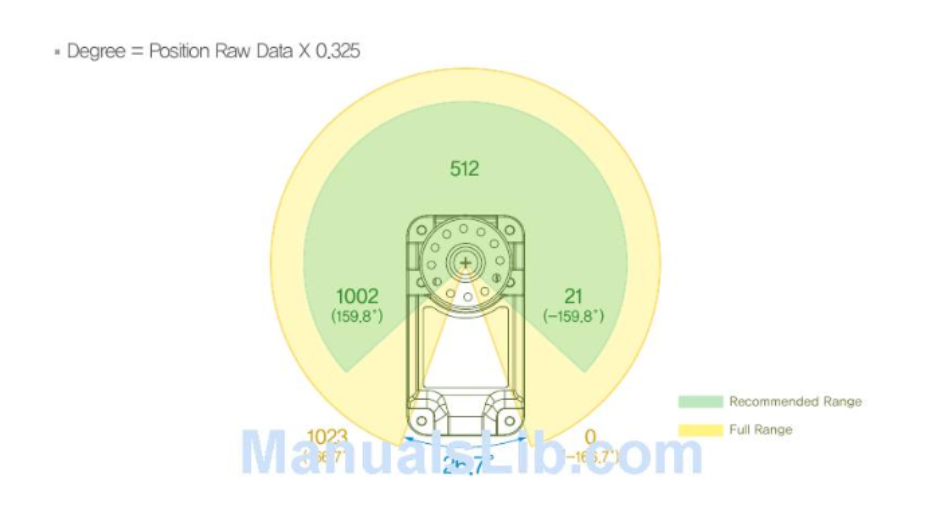
\includegraphics[width=0.8\textwidth]{../images/ServomoteurDegree}
	\caption{Shéma des positions angulaire du Servomoteur}
	\label{fig:SPAS}
\end{figure}

Ce servomoteur embarque un microcontrôleur qui lui permet d’avoir plusieurs
fonctionnalités comme :

\begin{itemize}
\item Un auto-diagnostique lui permettant la détection de surchauffe, la surcharge (si un obstacle le bloque lorsqu’il est en mouvement) et erreur de position
\item Retour d’état : il peut retourner la position, la tension et la température
\end{itemize}

\textbf{Pourquoi utilise-t-on ce servomoteur ?}

Dans le cadre du projet on utilise principalement ces servomoteurs car ils sont chainables, ce qui facilite les branchements si on souhaite en utiliser plusieurs, ce qui est le cas pour ce projet. La communication se fait à l’aide de 2 câbles, TX qui permet la transmission de données et RX qui permet la réception de données. De plus chaque servomoteur possède une adresse (ID) qui peut le rendre unique allant de 0 à 253.

\begin{figure}[H]
	\centering
	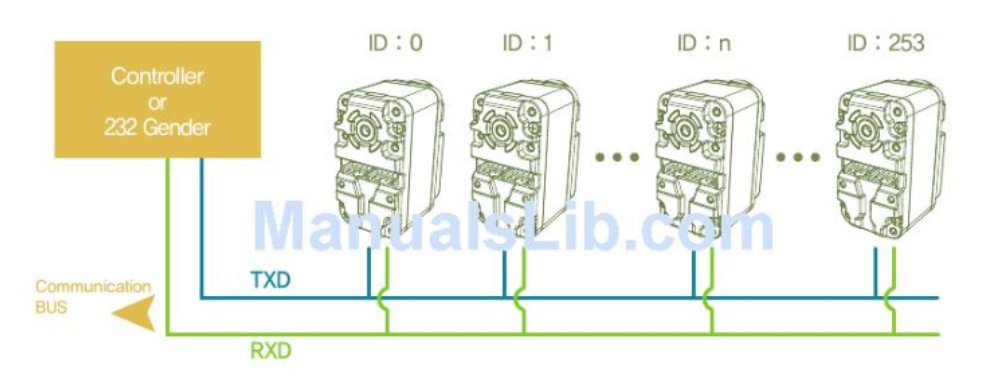
\includegraphics[width=0.8\textwidth]{../images/ServomoteurChain}
	\caption{Shéma du chainages des Servomoteurs}
	\label{fig:SCS}
\end{figure}

Donc la communication se fait via un protocole série qui envoie une trame de données où l’on renseigne la taille de la trame, l’ID auquel s’adresse la trame, la commande, le checksum qui vérifie les potentielles erreurs lors de la transmission de la trame et les données, comme la position.

\begin{figure}[H]
	\centering
	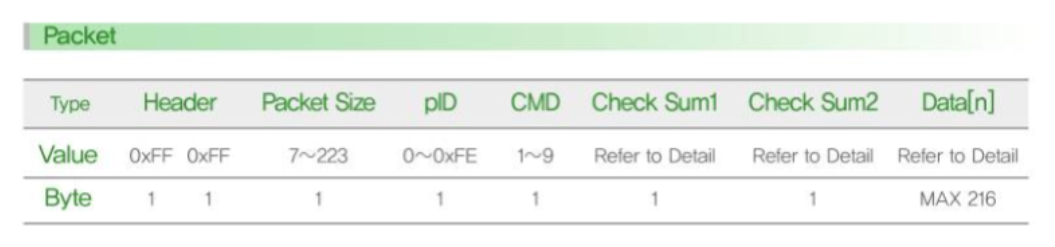
\includegraphics[width=0.8\textwidth]{../images/ServomoteurTab}
	\caption{Shéma des trames du Servomoteurs}
	\label{fig:STS}
\end{figure}

\subsubsection{Test Unitaire}

Avant de passer directement au code j’ai fait des petites vérifications me permettant de vérifier que le matériel fonctionnait correctement. Pour cela j’ai utilisé un logiciel qui n’est plus téléchargeable aujourd’hui qui m’a permis de scanner la voie série me permettant de détecter les servomoteurs connectés. Ensuite j’ai utilisé les méthodes de la classe qui m’a été fournis afin de vérifier si les servomoteurs fonctionnés.

\textbf{Description de la classe ServoH}

La classe ServoH à pour objectif de contrôler les servomoteurs Herkulex via le port UART de la raspberry.

Constructeurs :

\begin{itemize}
\item ServoH(serialib* VS, uint8\_t id) : Initialise le servo avec un pointeur vers l’objet de communication série serialib, un identifiant id, et des paramètres par défaut (vitesse, position, mode, couple...)
\item ServoH() : Constructeur vide, initialise les attributs servoCasiers et servoRFID à 0
\item ServoH(serialib* VS) : Initialise uniquement l’interface série
\end{itemize}

Méthodes de communication / gestion de bus :

\begin{itemize}
\item scanServos(serialib* VS) : Scanne le bus série pour détecter les servos connectés et affiche leurs ID
\item openConnection(const std::string\&amp; port, int baudrate, serialib\&amp; VS) : Ouvre une connexion série sur un port avec un débit donné
\item closeConnection(serialib\&amp; VS) : Ferme la connexion série
\end{itemize}

\textbf{Lecture et statut}

\begin{itemize}
\item readStatusServo(uint16\_t status, ServoH\&amp; s) : Lit l’état du servo passé en paramètre et affiche le statut brut et décomposé (haut/bas bits)
\item getservoCasiers() / getservoRFID() / getservoTest() : Accesseurs pour les seuils de tension associés aux servos spécifiques
\item readInfoServoTXT() : Lit un fichier texte contenant des données de configuration de servos et remplit les seuils (servoCasiers, servoRFID, test) et des positions
\end{itemize}

\textbf{Actions sur le servo :}

\begin{itemize}
\item openServo() / closeServo() : Ouvrir ou fermer un servo en position, active le couple, place à un angle, attend un certain temps
\item openServoTestVolt() / closeServoTestVolt() : Similaire, mais mesure la tension pendant le mouvement pour détection d’anomalies (ex. : surconsommation)
\item openRfidServo() / closeRfidServo() : Actions spécifiques à un servo contrôlant un mécanisme RFID, utilisant son propre seuil
\item stopServo(ServoH s, float typeServo) : Arrête le servo si la tension passe sous le seuil (typeServo). Affiche la position et tension
\end{itemize}

\textbf{Commandes Herkulex :}

\begin{itemize}
\item sendSimpleIJOGData() : Envoie une commande simple IJOG pour positionner le servo
\item writeEEPROM() / writeRegs() : Écrit dans les registres EEPROM ou RAM du servo
\item readEEPROM() / readRAM() / readRegs() : Lecture des registres EEPROM ou RAM
\item recvFrame() : Réception d’une trame de données depuis le servo
\end{itemize}

\textbf{Utilitaires \& configuration :}

\begin{itemize}
\item init() : Initialise les données du servo (plages de position, mode de contrôle, position actuelle)
\item changeID(oldId, newId) : Change l’ID du servo dans l’EEPROM
\item fixNewId() : Méthode appelée par changeID() qui écrit la nouvelle ID
\item fixTorque(HERKULEX\_TORQUE\_VALUE torque) : Modifie la valeur de couple appliquée par le servo (activé, libre, etc.)
\item fixPosition() / fixDegree() : Change la position du servo (en unités internes ou en degrés)
\item convertPositionToDegree(int position, const int midPosition) : Conversion d'une position interne à un angle (0.325 °/unité)
\item ServoValuePos readInfoServoPos() : Lit le fichier texte puis récupère la position des servomoteurs
\item ServoValueVolt readInfoServoVolt() : Lit le fichier texte puis récupère la tension des servomoteurs
\item void changeTXT(float val, string text, string idservo) : permet de modifier les informations du fichier texte
\end{itemize}

Vérification / Validation :

\begin{itemize}
\item calcCRC1() / calcCRC2() : Calcule les sommes de contrôle (CRC) utilisées dans les trames Herkulex
\item getId() : Retourne l’ID du servo
\end{itemize}

Variables membres (utilisées ou manipulées) :

\begin{itemize}
\item serialib* VS : Pointeur vers l’interface série
\item uint8\_t id : ID unique du servo
\item uint16\_t position : Position actuelle
\item HERKULEX\_CONTROL\_MODE controlMode : Mode (position ou vitesse)
\item HERKULEX\_TORQUE\_VALUE torque : État du couple.
\item std::string errorMessage : Messages d’erreurs cumulés
\item vector\&lt;uint8\_t\&gt; frameToSend / frameRecv : Buffers pour la communication série
\end{itemize}


\subsubsection{Description de la classe ServoH}

La classe ServoH à pour objectif de contrôler les servomoteurs Herkulex via le port UART de la raspberry.
 
\textbf{Constructeurs :}

\begin{itemize}
\item ServoH(serialib* VS, uint8\_t id) : Initialise le servo avec un pointeur vers l’objet de communication série serialib, un identifiant id, et des paramètres par défaut (vitesse, position, mode, couple...)
\item ServoH() : Constructeur vide, initialise les attributs servoCasiers et servoRFID à 0
\item ServoH(serialib* VS) : Initialise uniquement l’interface série
\end{itemize}
 
 
\textbf{Méthodes de communication / gestion de bus}

\begin{itemize}
\item scanServos(serialib* VS) : Scanne le bus série pour détecter les servos connectés et affiche leurs ID
\item openConnection(const std::string\& port, int baudrate, serialib\& VS) : Ouvre une connexion série sur un port avec un débit donné
\item closeConnection(serialib\& VS) : Ferme la connexion série
\end{itemize}
 
\textbf{Lecture et statut}

\begin{itemize}
\item readStatusServo(uint16\_t status, ServoH\& s) : Lit l’état du servo passé en paramètre et affiche le statut brut et décomposé (haut/bas bits)
\item getservoCasiers() / getservoRFID() / getservoTest() : Accesseurs pour les seuils de tension associés aux servos spécifiques
\item readInfoServoTXT() : Lit un fichier texte contenant des données de configuration de servos et remplit les seuils (servoCasiers, servoRFID, test) et des positions
\end{itemize}

\textbf{Actions sur le servo}

\begin{itemize}
\item openServo() / closeServo() : Ouvrir ou fermer un servo en position, active le couple, place à un angle, attend un certain temps
\item openServoTestVolt() / closeServoTestVolt() : Similaire, mais mesure la tension pendant le mouvement pour détection d’anomalies (ex. : surconsommation)
\item openRfidServo() / closeRfidServo() : Actions spécifiques à un servo contrôlant un mécanisme RFID, utilisant son propre seuil
\item stopServo(ServoH s, float typeServo) : Arrête le servo si la tension passe sous le seuil (typeServo). Affiche la position et tension
\end{itemize}
 
\textbf{Commandes Herkulex}

\begin{itemize}
\item sendSimpleIJOGData() : Envoie une commande simple IJOG pour positionner le servo
\item writeEEPROM() / writeRegs() : Écrit dans les registres EEPROM ou RAM du servo
\item readEEPROM() / readRAM() / readRegs() : Lecture des registres EEPROM ou RAM
\item recvFrame() : Réception d’une trame de données depuis le servo
\end{itemize}

\textbf{Utilitaires \& configuration}

\begin{itemize}
\item init() : Initialise les données du servo (plages de position, mode de contrôle, position actuelle)
\item changeID(oldId, newId) : Change l’ID du servo dans l’EEPROM.
\item fixNewId() : Méthode appelée par changeID() qui écrit la nouvelle ID
\item fixTorque(HERKULEX\_TORQUE\_VALUE torque) : Modifie la valeur de couple appliquée par le servo (activé, libre, etc.)
\item fixPosition() / fixDegree() : Change la position du servo (en unités internes ou en degrés)
\item convertPositionToDegree(int position, const int midPosition) : Conversion d'une position interne à un angle (0.325 °/unité)
\item ServoValuePos readInfoServoPos() : Lit le fichier texte puis récupère la position des servomoteurs
\item ServoValueVolt readInfoServoVolt() : Lit le fichier texte puis récupère la tension des servomoteurs
\item void changeTXT(float val, string text, string idservo) : permet de modifier les informations du fichier texte
\end{itemize}

\textbf{Vérification / Validation}

\begin{itemize}
\item calcCRC1() / calcCRC2() : Calcule les sommes de contrôle (CRC) utilisées dans les trames Herkulex
\item getId() : Retourne l’ID du servo.
\end{itemize}
 
\textbf{Variables membres (utilisées ou manipulées)}

\begin{itemize}
\item serialib* VS : Pointeur vers l’interface série
\item uint8\_t id : ID unique du servo
\item uint16\_t position : Position actuelle
\item HERKULEX\_CONTROL\_MODE controlMode : Mode (position ou vitesse)
\item HERKULEX\_TORQUE\_VALUE torque : État du couple
\item std::string errorMessage : Messages d’erreurs cumulés
\item vector<uint8\_t> frameToSend / frameRecv : Buffers pour la communication série
\end{itemize}

\subsection{Projet final}

\subsubsection{Main}

Le main du projet final réuni la classe requête, RFID, servoH, DelRGBChainable et la base de données. Il a donc pour rôle d’ouvrir et de fermer les casiers en actionnant les servomoteur lorsqu’une carte rfid est scanner par le lecteur RFID uniquement si l’affectation de la carte est valide dans la base de données. Par exemple si l’affectation est carte « perdu » alors les servomoteurs ne sont pas censés s’actionner.

\textbf{Explication du Main :}

On commence par définir une fonction permettant de lire les positions des servomoteurs à partir d’un fichier texte, en extrayant uniquement les valeurs des lignes au format attendu.

Dans la fonction principale, plusieurs objets sont initialisés : une chaîne de LED RGB, des objets pour gérer les servos, la communication série, la lecture RFID, et la gestion de la base de données.

Le programme affiche les positions des servos lues initialement puis tente d’établir une connexion avec la base de données distante. Si cette connexion échoue, le programme s’arrête. De même, il tente ensuite d’ouvrir le port série du lecteur RFID, en arrêtant l’exécution en cas d’erreur.

Une fois les périphériques correctement initialisés, la connexion série avec les servos est ouverte. Le programme scanne ensuite le bus pour détecter les servomoteurs présents et affiche leurs identifiants. Des objets représentant plusieurs servos sont créés.

Le programme entre ensuite dans une boucle infinie dans laquelle il attend la lecture d’un badge RFID. Lorsque celui-ci est détecté, son identifiant est affiché et recherché dans la base de données. Si le badge est reconnu, un message est affiché, une LED verte est activée pour signaler que le badge est déjà enregistré, et le servo associé au casier correspondant est commandé pour s’ouvrir puis se fermer. Des effets lumineux alternant vert et rouge sont ensuite réalisés plusieurs fois sur la chaîne LED.

Si le badge n’est pas reconnu, une LED rouge est activée. Le servo 0 est également actionné pour laisser passer la carte RFID.

Enfin, lorsque le programme est terminé, les connexions série, GPIO, port RFID et base de données sont correctement fermées et libérées.

\begin{figure}[H]
	\centering
	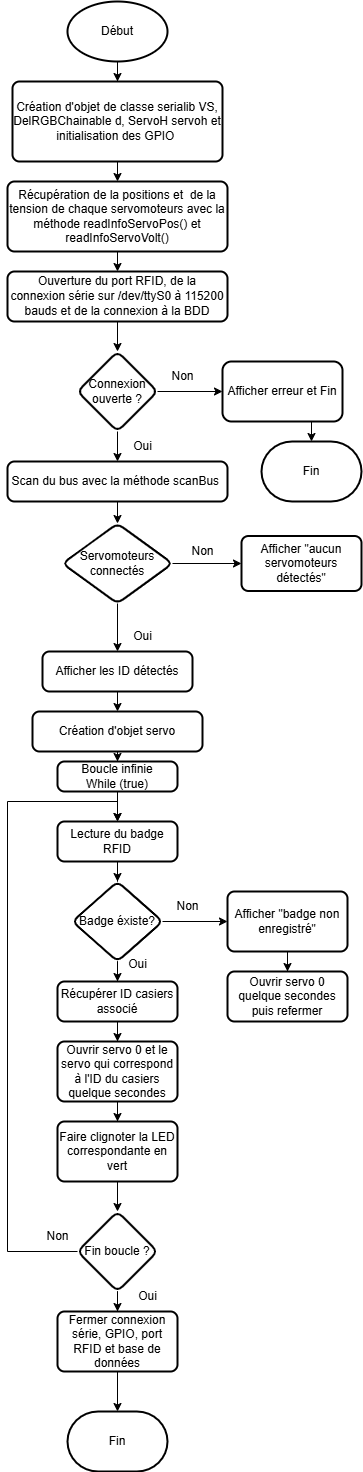
\includegraphics[width=0.35\textwidth]{../images/algoMainPin}
	\caption{Algorithme du Main}
	\label{fig:AMP}
\end{figure}

\subsection{Bonus}

\subsubsection{Modif\_servo.exe}

En cas de problème, si un servomoteur dysfonctionne par exemple, cet exécutable a pour objectif de permettre à un utilisateur de modifier l’identifiant (ID) d’un servomoteur connecté via une liaison série afin de remplacer le servomoteur défaillant par un nouveau. On commence par initialiser un objet de communication série « VS » ainsi qu’un objet représentant les fonctions associées aux servomoteurs « servoh ». Une connexion est ensuite établie sur le port série /dev/ttyS0 à une vitesse de 115200 bauds. Une fois connecté, on effectue un balayage du bus série pour détecter les servos présents, en stockant leurs identifiants dans un vecteur. Si des servos sont trouvés, leurs ID sont affichés. Sinon, un message signale qu’aucun servo n’a été détecté.

L'utilisateur est ensuite invité à interagir dans une boucle. Il peut entrer l’ID actuel d’un servomoteur et spécifier un nouvel ID à lui attribuer. À tout moment, il peut saisir "exit" pour quitter la boucle. On vérifie que l’ancien ID saisi correspond bien à un servo détecté. Si ce n’est pas le cas, un message d’erreur s’affiche et l’utilisateur est invité à réessayer. Si l’ID est valide, un objet représentant le servomoteur ciblé est créé, puis la commande de changement d’ID est exécutée via la méthode changeID(oldId, newId).

Une fois l'utilisateur sorti de la boucle, la connexion série est fermée proprement, et le programme se termine.

\begin{figure}[H]
	\centering
	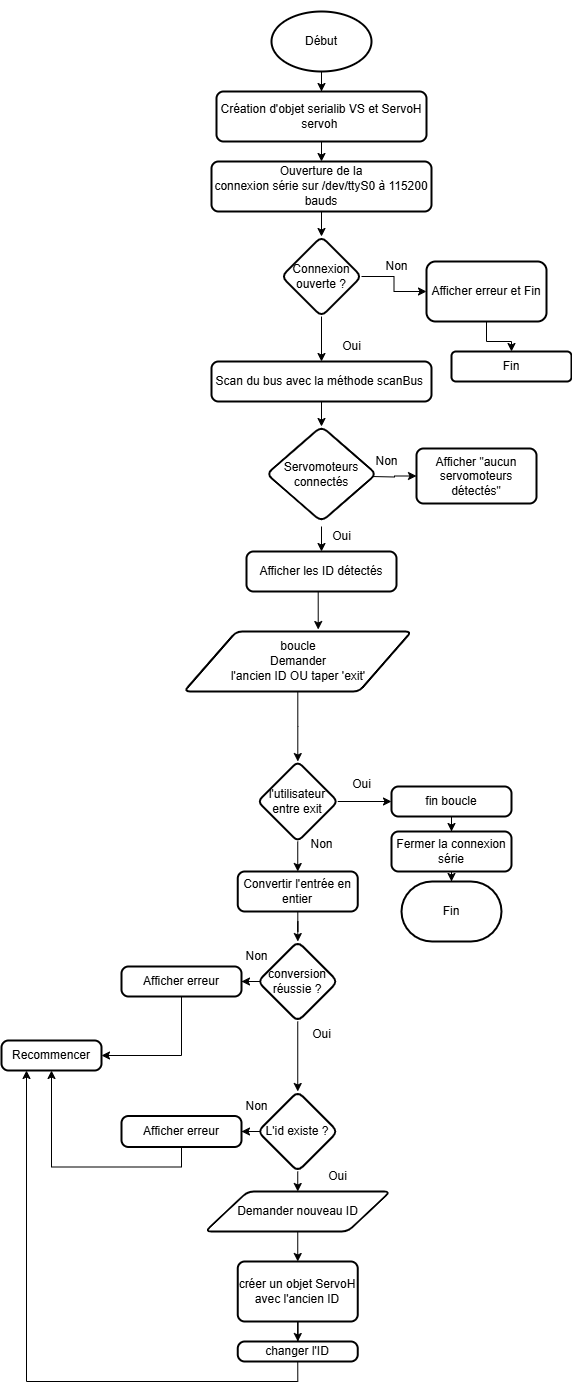
\includegraphics[width=0.6\textwidth]{../images/algoModifServo}
	\caption{Algorithme de Modif\_servo.exe}
	\label{fig:AM}
\end{figure}

\subsubsection{Pos\_servo.exe}

En cas de changement de servomoteur, cet exécutable a pour objectif d’enregistrer dans un fichier texte la position de fermeture du nouveau servomoteur. Car en fonction de comment ils sont montés, la position peut varier d’un servo à l’autre. Pour bien exécuter le code il faut que le servomoteur en question soit en position de fermeture. On commence par créer les objets nécessaires à la communication série et au contrôle des servomoteurs. Ensuite, on affiche un message indiquant que l’on va ouvrir la connexion série. On tente alors d’ouvrir cette connexion sur le port spécifié avec la vitesse de transmission définie. Si l’ouverture échoue, on affiche un message d’erreur et on termine le programme. Dans le cas contraire, on confirme que la connexion est bien établie.

Puis, on réalise un scan du bus pour détecter les servos connectés. Si le scan échoue, on affiche un message d’erreur, on ferme la connexion série et on termine le programme. Si le scan réussit, on affiche un message indiquant que le scan est terminé.

Pour chaque servo détecté, on crée un objet représentant ce servo avec son identifiant, puis on tente de lire sa position actuelle. Si la lecture réussit, on convertit la position en degré selon une formule donnée, puis on affiche l’identifiant du servo ainsi que sa position et la valeur correspondante en degrés. Si la lecture échoue, on affiche un message d’erreur précisant le problème rencontré.

Enfin, après avoir traité tous les servos détectés, on ferme proprement la connexion série avant de terminer l’exécution du programme.

\begin{figure}[H]
	\centering
	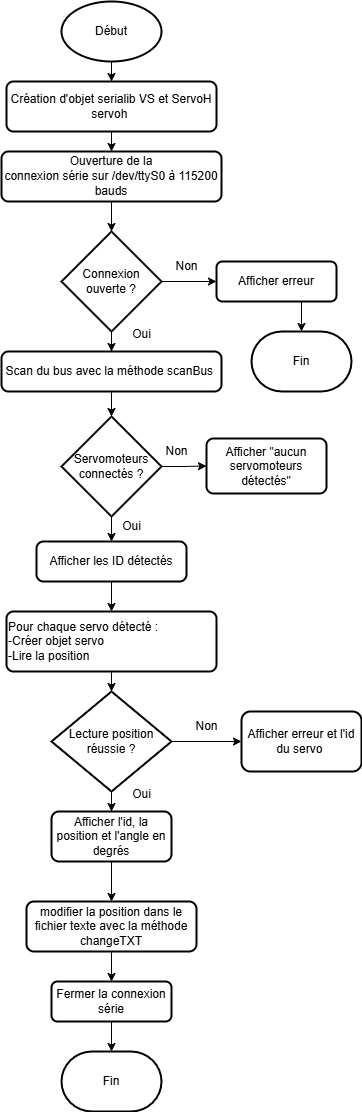
\includegraphics[width=0.45\textwidth]{../images/algoDegreeServo}
	\caption{Algorithme de Pos\_servo.exe}
	\label{fig:AP}
\end{figure}

\subsubsection{Volt\_servo.exe}

Les servomoteurs ont un système de sécurité capable d’arrêter le mouvement du servomoteur si quelque chose ou quelqu’un bloque son ouverture ou sa fermeture, comme une main par exemple. Ce système ce base sur la tension du servomoteur, si elle diminue anormalement alors un obstacle empêche le servomoteur de s’ouvrir ou de se fermer correctement. Cet exécutable a donc pour objectif de vérifier la tension minimale du servomoteur lors de son ouverture et de sa fermeture puis de l’enregistrer dans un fichier texte. Comme ça lorsque le servomoteur dépassera cette tension il s’arrêtera.

On commence par créer les objets nécessaires à la communication avec les servos et à la gestion des valeurs lues. On affiche ensuite les valeurs initiales des servos disponibles, puis on lit les informations de configuration des servos depuis un fichier texte pour mettre à jour ces valeurs. Ces valeurs mises à jour sont affichées.

On affiche un message indiquant que l’on va ouvrir la connexion série, puis on tente d’établir cette connexion sur le port et le débit définis. Si la connexion ne peut pas être ouverte, on affiche un message d’erreur et on arrête le programme. Sinon, on confirme que la connexion est bien établie.

On affiche un message avant de lancer un scan du bus pour détecter tous les servos connectés. Si des servos sont détectés, on affiche leurs identifiants. Sinon, on indique qu’aucun servo n’a été trouvé.

Ensuite, on entre dans une boucle d’interaction avec l’utilisateur qui peut choisir de tester un servo en entrant son identifiant ou de quitter en tapant "exit". Pour chaque entrée utilisateur, on vérifie que celle-ci est convertible en nombre et que l’identifiant correspond bien à un servo détecté sur le bus. En cas d’erreur, on informe l’utilisateur et on lui demande une nouvelle saisie.

Quand un identifiant valide est sélectionné, on crée un objet servo correspondant, puis on récupère la position en degrés de ce servo à partir des données précédemment lues. On réalise alors des tests de tension minimale, d’abord avec le servo en position ouverte, puis en position fermée, en affichant les résultats à chaque étape.

Pour s’assurer de la stabilité des mesures, on effectue une série d’appels répétés aux fonctions de test de tension pendant environ cinq secondes. Une fois le test terminé, on affiche un message indiquant la fin du test et la tension minimale mesurée.

La boucle recommence tant que l’utilisateur ne choisit pas de quitter. Lorsque celui-ci tape "exit", la boucle se termine, on ferme proprement la connexion série et on termine le programme.

\begin{figure}[H]
	\centering
	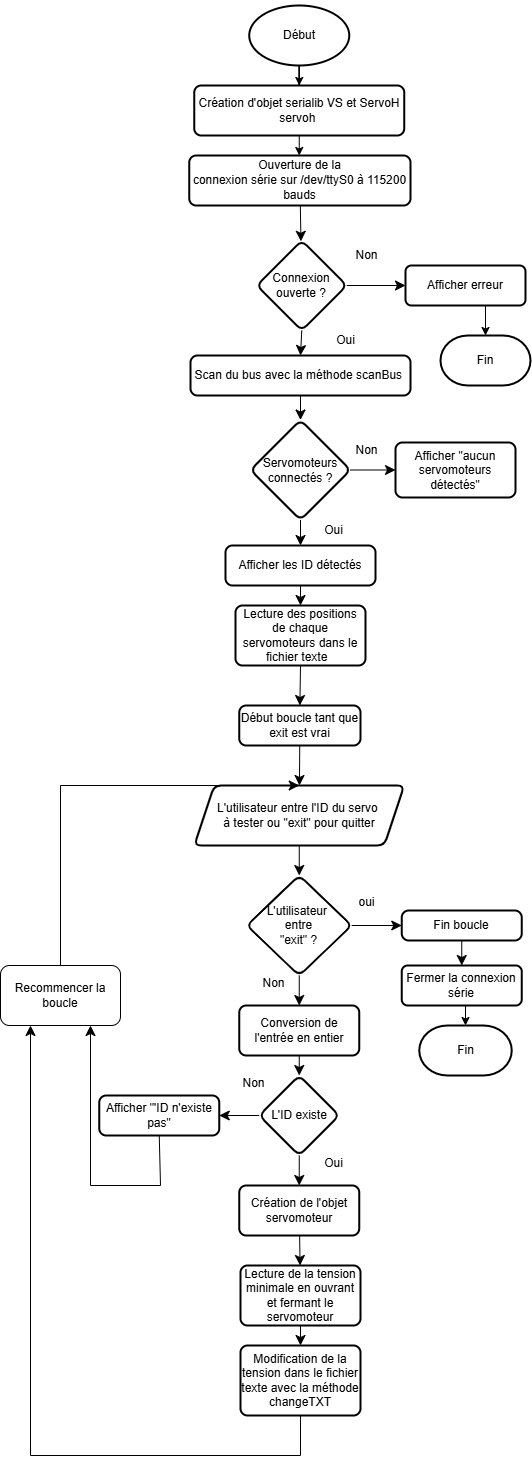
\includegraphics[width=0.5\textwidth]{../images/algoVoltServo}
	\caption{Algorithme de Volt\_servo.exe}
	\label{fig:AV}
\end{figure}

\newpage

\end{document}